\section{Application to the COVID-19 outbreak}

The model described in Section~\ref{sec:model} is tuned here to fit at best the dataset from Lombardy shown in Figure~\ref{fig:data_lombardy}. Since the data available show just the leading curve of the outbreak, only parameters $\beta$, $\braket{k}$, $\delta$ and $\tau$ have to be tuned. Moreover, an additional parameter $t_0$ has been added to shift the distribution in time. The available dataset regards the \emph{total cases}, corresponding to the sum of infected (positively tested), recovered and deaths. This is not immediately comparable with the population classes in the model. Here it is identified as the sum of quarantined, recovered and deaths. Infected population is not included in the total number because it would correspond to the whole infected population being tested as positive, even the population not showing symptoms, highly probable in young population. Therefore the infected population correspond to the part of the population that has the virus but has not been tested, and all the positively tested population is immediately quarantined. The best fitting setup is shown in Figure~\ref{fig:data_vs_model_first_lombardy}. Parameters modifying the trailing edge of the infection is set to approximate values of the outbreak. Mortality is set to $2\%$, reinfection probability to $10^{-5}$ since yet no cases have been observed. Population is set to $10^7$, corresponding to Lombardy population.\\

\begin{figure}
\centering
  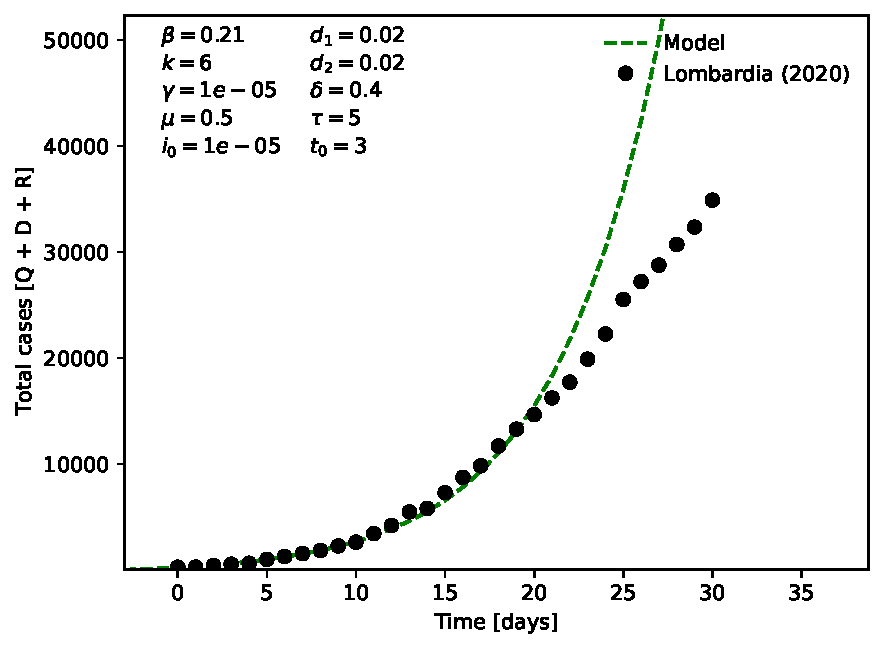
\includegraphics[width=0.4\textwidth]{imgs/Covid/DataVsModel_parameters_Lombardia_less_impacting.pdf}
  \caption{Best match of parameters to make the model described in Section~\ref{sec:model} fit with data il Lombardy.}
  \label{fig:data_vs_model_first_lombardy}
\end{figure}

As shown in Figure~\ref{fig:data_vs_model_first_lombardy} the model predicts an exponential growth until reaching a peak, that is not what is measured, since different slopes in the total cases curves are present. Possibly this is due to changing in the small-world conditions such as limitation to the social activity (mandatory closings of shops, cancellations of events, etc.), improvements of the sanitary checking and testing. This should cause a decrease of the slope, instead of an increase, caused, for example, by a longer incubation time. This hypothesis is quite encouraged by the dates on data when the change of slopes occur: around March 10th and 20th. On March 9th and 11th two special laws have been approved and applied, closing all shops, limitation of movements for citizens. On March 10th even a tighter regulation have been introduced: no movements among cities and mandatory closing of all the activities except for hospital, farmacies, hostera and corresponding chains. The corona virus' incubation time, although the recommended quarantine of fifteen days, it has a shorter incubation time before possible symptoms happen of less than a week. Therefore the effects of the actions affect the curve in few days.\\

The idea to adapt the model to the real world scenario, two improvements have been implemented:
\begin{itemize}
\item Scheduling of $\delta$ parameter: this reflects the different sanitary and testing coverage versus time.
\item Scheduling of $\braket{k}$ parameter: this reflects the change in social activiti in time.
\item {color{red}Fluctuation of $\delta$ parameter: this reflects the fluctuation of the number of tests done per day.}
\end{itemize}


\section{Improvement of the model}
Here the scheduling of the parameters is described. The $\delta$ parameter regulates the fraction of infected people that is positively tested and quarantined. The tests and quarantine pressure has been increased in time, following a trend similar to Figure~\ref{fig:scheduling}. This estimation is based on the trend followed by the total number of tests performed against time, passing from $10\%$ to $100\%$ of the current number in ten days. The maximum cover is given by the set $\delta$ parameter in input to the simulation. The $\braket{k}$ scheduling represents the limitation of the social interactions, from a freely-communicating system to isolation where an infected person may interact only with a susceptible individual.

\begin{figure}
\centering
  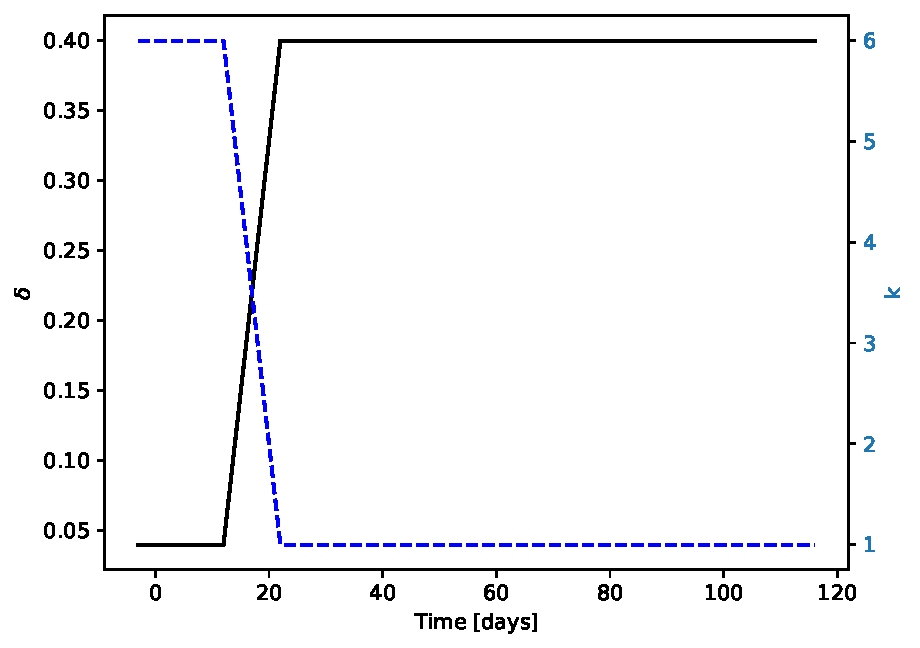
\includegraphics[width=0.4\textwidth]{imgs/Covid/Scheduling.pdf}
  \caption{Scheduling of $\delta$ and $\braket{k}$ parameters in time. The reference values of the parameters are set the same as in Figure~\ref{fig:data_vs_model_first_lombardy}.}
  \label{fig:scheduling}
\end{figure}
